\documentclass[brasil]{abnt}
\usepackage[abnt-repeated-author-omit=yes]{abntcite}
\citebrackets[]

\usepackage[utf8]{inputenc}
\usepackage[brazil]{babel}
\usepackage{graphicx}
\usepackage{amsmath}
\usepackage{amsfonts}
\usepackage{listings}
\usepackage{url}

\begin{document}

    \autor{Amanda Piaceski Arceno}
    \titulo{O ensino de matemática para alunos surdos: Reflexões a partir de uma breve revisão bibliográfica}
    \orientador[Orientadora:\\]{Janine Soares de Oliveira}
    \comentario{Trabalho de Conclusão de Curso apresentado como parte dos requisitos para obtenção da graduação em Matemática Licenciatura do Departamento de Matemática do Centro de Ciências Físicas e Matemáticas da 
				Universidade Federal de Santa Catarina, sob a orientação da Profª Dra. Janine Soares de Oliveira.}
    \instituicao{Departamento de Matemática \par Centro de Ciências Físicas e Matemáticas \par Universidade Federal De Santa Catarina}
    \local{Florianópolis - SC, Brasil}
    \data{03 de dezembro 2015}

\capa
\folhaderosto

\begin{folhadeaprovacao}
    Trabalho de Conclusão de Curso apresentado como parte dos requisitos para obtenção da graduação em Matemática Licenciatura do Departamento de Matemática do Centro de Ciências Físicas e Matemáticas da 
	Universidade Federal de Santa Catarina, sob a orientação da Profa Dra. Janine Soares de Oliveira.

\setlength{\ABNTsignthickness}{0.4pt}

    \assinatura{Profª. Dra. Janine Soares de Oliveira\\ Universidade Federal de Santa Catarina\\ Orientadora}
    \assinatura{Profª. Ma. Débora Campos Wanderley\\ Universidade Federal de Santa Catarina}
    \assinatura{Prof. Me. Nereu Estanislau Burin\\ Universidade Federal de Santa Catarina}
    
\end{folhadeaprovacao}


\chapter*{Agradecimentos}

	Agradeço inicialmente a minha mãe Nilsa e minha avó Erna que me forneceram muito mais do que o
	necessário para ser capaz de realizar esta consquista. Que me acompanharam em cada etapa e
	cujo orgulho sempre foi, e sempre será, motivo mais do que suficiente para ter força e conquistar 
	qualquer coisa em minha vida. Pelo apoio incansável em cada momento de minha graduação,
	agradeço meu esposo Marcos que me inspira a querer ser alguém melhor a cada dia.
	
	A professora Janine pela oportunidade de realizar um trabalho tão prazeroso.

\begin{resumo}
	Este trabalho tem como função mostrar a importância de um novo olhar a respeito da educação e do ensino de alunos surdos, bem como o ensino e a aprendizagem de alunos surdos com
	relação a disciplina de matemática. O objetivo é defender a educação bilíngue, prezando o uso da Libras - Língua Brasileira de Sinais, primeira língua dos surdos, como um meio de comunicação entre estes sujeitos 
	e da Língua Portuguesa, segunda língua, como linguagem escrita. O presente trabalho, de cunho investigativo, visa através de pesquisas, esclarecer as leis brasileiras aplicadas à 
	educação  de surdos, defender o papel do aluno surdo em uma sala de aula onde a maioria dos alunos é ouvinte, investigar como se constituiu ao longo do tempo a educação de alunos 
	surdos no Brasil e as filosofias educacionais pensadas ao longo dos séculos na educação de alunos surdos. Por fim, o presente trabalho tem como finalidade mostrar se alunos surdos
	são capazes de compreender ou não conceitos matemáticos e se podem apresentar habilidades ou não em matemática.   
	
	Palavras chaves: Educação de Surdos - Educação Bilíngue - Ensino de Matemática  

\end{resumo}

\tableofcontents

\chapter*{Introdução}
	
	Ao refletir sobre o papel da escola como  espaço de desenvolvimento, ambiente socializador e formador, e do ofício do professor enquanto educador surgiu o desejo pela investigação
	sobre a educação de alunos surdos, suas capacidades e/ou suas habilidades, sua história educacional, as politicas educacionais brasileiras, as filosofias educacionais pensadas para estes alunos
	ao longo dos séculos, o ensino e a aprendizagem de matemática para estes alunos.  
		
	Conforme a lei nº 9.394, de 20 dezembro de 1996, a educação escolar 
	deve abranger os processos formativos vinculadas à prática social e 
	ao mundo do trabalho. E ainda, o ensino destes alunos devem seguir 
	os princípios de: igualdade de condições para o acesso e a 
	permanência na escola; liberdade de aprender, ensinar, pesquisar e 
	divulgar a cultura, o pensamento, a arte e o saber; pluralismo de 
	ideias e de concepções pedagógicas; respeito à liberdade e apreço 
	a tolerância; coexistência de instituições públicas e privadas de 
	ensino; gratuidade do ensino público em estabelecimentos oficiais; 
	valorização do profissional da educação escolar;  
	garantia de padrão de qualidade; valorização da experiência 
	extra-escolar; vinculação entre a educação escolar, o trabalho e 
	as práticas sociais; e consideração com a diversidade étnico-racial.  
	
	A escola é um espaço onde se desenvolve a educação e tem como função a preservação, a transformação cultural e o desenvolvimento do aluno. 
	Neste sentido, para um aluno surdo ter acesso à educação em uma classe inclusiva 
	\footnote{A educação inclusiva se constitui da diversidade dos 
	indivíduos, buscando perceber e atender as necessidades de todos os 
	estudantes, em salas de aulas comuns, em um sistema inclusivo de 
	ensino, de forma a promover a aprendizagem e o desenvolvimento 
	social de todos.}
	da rede regular de ensino, faz-se necessário um profissional que 
	traduza e interprete - tradutor/intérprete
	\footnote{O Tradutor e intérprete faz a transposição do significado de textos e de falas de um idioma para outro.}
	- os conhecimentos que 
	estão sendo proporcionados nesse ambiente para este aluno surdo, através da língua de sinais
	\footnote{Língua de sinais ou língua gestual é uma língua que utiliza gestos, sinais e expressões faciais e corporais, em vez de sons na comunicação.}.
	
	A escola tem sua participação no movimento de transformação da sociedade, a partir de abordagens pode-se desenvolver o que lhe é específico, a garantia de acesso 
	ao saber e do exercício crítico da cidadania. 
	
	Antes do século XIX, os surdos ocupavam papeis significativos na sociedade, sua educação seguia por meio da língua de sinas e os professores destes alunos, na sua grande maioria, eram surdos. Porém, 
	haviam muitas divergências a respeito deste método. Uns defendiam que a maneira mais indicada para se ensinar um aluno surdo seria através da linguagem oral, outros através da língua de sinais e outros, 
	pelo método combinado (linguagem oral e língua de sinais). Como 
	consta em documento produzido pelo MEC - \textit{Saberes e práticas da 
	inclusão: desenvolvendo competências para o atendimento às 
	necessidades educacionais especiais de alunos surdos}:
		
		\begin{citacao} Em 1880, no Congresso Mundial de Professores de Surdos (Milão-Itália) 
						chegou-se à conclusão de que os surdos deveriam ser ensinados pelo método oral puro, sendo proibida a utilização da língua de sinais. A partir daí, a opressão de mais de 
						um século a que os surdos foram submetidos, sendo proibidos de utilizar sua língua e obrigados a comportarem-se como os ouvintes, trouxe uma série de consequências sociais 
						e educacionais negativas. (ARANHA et al, 2006, p.67).
		\end{citacao}

	Atualmente, há surdos que frequentam instituições escolares com enfoque oral, há os que frequentam instituições escolares que fazem uso da língua de sinais, os que nunca tiveram acesso à escola e os 
	que fazem parte de "movimentos de surdos" que lutam pelos seus direitos linguísticos. Há, ainda, os que falam o português oral e se adaptam a tal forma de comunicação, porém, não há um grupo homogêneo. 	
	
	O conhecimento da Língua Brasileira de Sinais para estudantes de cursos de licenciatura se tornou muito importante, tendo em vista a inclusão de alunos surdos em classes de escolas onde a maioria dos alunos é ouvinte. 
	Vale lembrar que, o papel do professor enquanto educador é o de ensinar os alunos a pensar, a questionar e a aprender a viver em sociedade, para que possam construir opiniões próprias. Portanto, a educação e o ensino de
	alunos surdos não deve ser vista de maneira diferente dos demais alunos.
	
	Diante disto, este trabalho tem como propósito estudar pressupostos 
	teóricos que permeiam os conceitos relacionados com a educação 
	matemática para alunos surdos. Teóricos como Peixoto (2013), Cruz 
	e Lautert (2014), Sales (2013) e Leite (2007) irão, dentre outros autores, subsidiar essa pesquisa, pois destacam em suas obras aspectos que dizem respeito à educação dos surdos; a relação dos surdos com os ouvintes nos ambientes 
	escolares, conceitos como diferença e deficiência, maioria e minoria, linguagem oral e língua escrita; a importância do uso da língua de sinais na construção da identidade surda, constituindo assim a comunidade
	surda; o processo de transformação ao longo tempo em relação a educação de surdos; a educação bilíngue; filosofias educacionais no ensino e na aprendizagem de estudantes surdos, bem como a formação de professores para 
	o ensino destes sujeitos; e por fim, reflexões sobre a educação e o ensino de matemática para alunos surdos. 
	
	Assim, este trabalho tem como objetivo geral levantar, através de documentos estudados, reflexões sobre o ensino e aprendizagem de matemática para alunos com surdez. 
	Para tanto, os objetivos são: identificar como se constitui a educação brasileira de surdos e as leis que a regem, e apontar as práticas educacionais aplicadas na educação de surdos e suas representações sociais sobre a 
	surdez. O objetivo desta pesquisa se deu através da seguinte problematização: Quais as filosofias educacionais já aplicadas na educação de alunos surdos em relação ao ensino e na aprendizagem de matemática?  
	
	A escolha do tema para a elaboração deste trabalho, o ensino de matemática para alunos surdos, se justifica por duas razões. A primeira pela elaboração de um projeto de ensino na 
	disciplina de Projetos II, da oitava fase, onde elaborei um projeto de pesquisa com o tema \textit{Pensando a prática docente da matemática na educação de alunos surdos}, este projeto visava a importância 
	da disciplina LIBRAS - Língua Brasileiras de Sinais na graduação do curso de Licenciatura em Matemática. A segunda razão pela qual me motivei a buscar informações a respeito deste tema, foi as reflexões 
	com relação a experiência de compor a turma da disciplina Língua Brasileira de Sinais, também na oitava fase do curso de Licenciatura em Matemática da UFSC - Universidade Federal de Santa Catarina, no ano 
	de 2012, onde, nesta turma, pude ter contato direto com pessoas surdas, dos quais eram professores desta disciplina, e da dificuldade que enfrentei em me comunicar com estes professores surdos. 
	
	Posto isto, o presente estudo está estruturado da seguinte maneira: A \textit{Política Nacional de Inclusão} - na qual tem a finalidade de mostrar as mudanças nas leis brasileiras ocorridas ao logo dos 
	tempos, bem como a luta dos surdos pelo reconhecimento da sua modalidade de comunicação, e ainda, o pensar o trabalho educativo desde os diferentes campos do conhecimento de forma a pensar a prática 
	inclusiva. \textit{O Educando surdo} - este ponto do estudo tem como objetivo esclarecer qual a diferença entre deficiente auditivo e surdo, ressaltar a importância do reconhecimento da Língua Brasileira de Sinais 
	perante a comunidade surda, como se constitui a língua de sinais e como surgiu a Língua Brasileira de Sinais. A \textit{História da educação de surdos} - este tem como finalidade contar um pouco 
	de como surgiram os primeiros estudos a respeito da educação de surdos, bem como a reflexão a respeito da inclusão de alunos surdos em ambientes escolares onde a maioria de alunos é ouvinte. As 
	\textit{Filosofias educacionais} - neste a finalidade é a de mostrar de forma detalhada as filosofias de ensino já vivencias por surdos no decorrer dos séculos, para isto, serão analisadas as abordagens oralista, 
	a comunicação total e o bilinguismo. A \textit{Educação Bilíngue} - tem a finalidade de mostrar como é a proposta bilíngue na educação de alunos com surdez. \textit{O ensino e a aprendizagem de Matemática} - tem como 
	objetivo trazer a reflexão a respeito da prática docente no ensino de matemática, bem como como a matemática é vista muitas das vezes. E ainda, tem como finalidade o esclarecimento de possíveis
	dúvidas com relação a capacidade de alunos surdos em compreender, ou ainda, de apresentar habilidades ou não na disciplina de matemática.  

\chapter{Política Nacional de Inclusão}
	A inclusão social levou a elaboração de políticas e leis na formação de programas e serviços voltados ao atendimento das necessidades especiais de pessoas com deficiência. Isto é, criar recursos que 
	adéquam estas pessoas aos sistemas sociais comuns e, em caso de inaptidão, criar-lhes adaptações para que possam participar ou acompanhar o ritmo dos demais. 
	
	A educação inclusiva está estabelecida nas \textit{Diretrizes Nacionais para a Educação Especial na Educação Básica}. Diretriz esta que garante o direito de acesso e permanência dos alunos com deficiência e orienta as instituições escolares para a integração destes sujeitos em classes do sistema inclusivo de ensino. Assim, uma criança com deficiência tem direito a cursar instituições 
	inclusivas, cabendo ao professor a iniciativa de elaborar e aplicar atividades propiciem um aprendizado adequado e que atendam as necessidades específicas destes alunos.
	Porém, sabemos que um professor sozinho pouco pode fazer diante da diversidade de questões que seus alunos apontam. 
		
	O Art. 3º do Decreto, de Nº 7.612 de 17 de novembro de 2011, garante um sistema educacional inclusivo onde os equipamentos públicos de educação sejam acessíveis para as pessoas com deficiência 
	inclusive por meio de transporte adequado; a ampliação da participação das pessoas com deficiência no mercado de trabalho, mediante sua capacitação e qualificação profissional; a 
	ampliação do acesso das pessoas com deficiência às políticas de assistência social e de combate à extrema pobreza; prevenção das causas de deficiência; ampliação e qualificação da rede de atenção à saúde 
	da pessoa com deficiência, em especial os serviços de habilitação e reabilitação; ampliação do acesso das pessoas com deficiência à habitação adaptável e com recursos de acessibilidade; e promoção do acesso, 
	do desenvolvimento e da inovação em tecnologia assistiva. 
						
	A lei Nº 13.146, de 6 de julho de 2015, \textit{Lei Brasileira de Inclusão da Pessoa com Deficiência}, em seu Art. 1º, assegura e promove, em condições de igualdade, o exercício dos direitos 
	e das liberdades fundamentais por pessoa com deficiência, visando à sua inclusão social e cidadania. Ainda, em seu Art. 2º, considera pessoa com deficiência aquela que tem impedimento de longo prazo de natureza 
	física, mental, intelectual ou sensorial, o qual, em interação com uma ou mais barreiras, pode obstruir sua participação plena e efetiva na sociedade em igualdade de condições com as demais pessoas. 
	
	Pensar o trabalho educativo desde os diferentes campos do 
	conhecimento, é fundamental para formar um prática inclusiva junto 
	ao professor. Como discorre Dutra no documento da \textit{Secretaria 
	de Educação Especial - Educação Inclusiva: A escola}:
	
		\begin{citacao} A falta de um apoio pedagógico a essas necessidades especiais pode fazer com que essas crianças e adolescentes não estejam na escola: muitas vezes as famílias não encontram escolas 
						organizadas para receber a todos e, fazer um bom atendimento, o que é uma forma de discriminar. A falta desse apoio pode também fazer com que essas crianças e adolescentes deixem a 
						escola depois de pouco tempo, ou permaneçam sem progredir para os níveis mais elevados de ensino, o que é uma forma de desigualdade de condições de permanência. 
						(ARANHA; DUTRA, 2004, p.4)
		\end{citacao}

	Sabe-se que a escola tem como compromisso propagar o saber universal e, como consequência, afim de alcançar seu objetivo, terá de saber lidar com o que há de particular na construção desse conhecimento. 
	Entretanto, haverá limitações naturais ao se tratar de alunos com deficiência. Tais limitações por si só, já apontam necessidade de existir um espaço, que não seja eminentemente facultativo, para esse fim.
	Como descrito por Paulon, Freitas e Pinto:
		
		\begin{citacao}Como território institucional expressivo da cultura em que se insere, a escola sofre pressões para acompanhar os novos tempos e lidar melhor com a diversidade do público que deve atender. 
						Um público de "aprendizes de cidadania" que, para exercê-la, querem mais que o mero direito de expressão. Mas também um público cheio de especificidades que, se não forem respeitadas, 
						acolhidas e atendidas em suas diferenças jamais farão da escola um dos possíveis espaços em que o exercício de uma política inclusiva contribua com a construção de uma sociedade mais 
						justa. (PAULON; FREITAS; PINTO, 2005, p. 7)
		\end{citacao}
	
	
	Seguindo esse sistema "de preferências" atribui-se, ainda que sem intenção, um sentimento de menor capacidade intelectual a alunos nos quais percebemos fragilidade, ritmo mais lento, 
	ou quaisquer outras características que os difiram dos demais alunos de uma turma. 
	Desta forma, é da competência do professor compreender as necessidades educacionais destes alunos e, assim, planejar os passos para uma intervenção cujo objetivo seja 
	alcançar uma aprendizagem efetiva.
	
	As escolas inclusivas devem propor um sistema educacional que considere as necessidades de todos os alunos e 
	deve estar de acordo com essas necessidades. 
 	A inclusão destes sujeitos causa uma mudança na perspectiva educacional, pois não se limita a ajudar somente os alunos que apresentam dificuldades na escola, mas apoia professores,
 	alunos e todos que compõem o corpo educacional, para que obtenham sucesso na fase escolar. 
		
	A inclusão ostenta uma proposta que tem como objetivo inserir e propagar o contato com as diferenças, o que parece ser algo que se enquadra na comunidade escolar. Entretanto os meios utilizados
	para promover esta inclusão não necessariamente são satisfatórios para aqueles que apresentam alguma necessidade especial, uma vez que carecem de uma série de condições as quais, na maioria das vezes, 
	não têm sido oferecidas pelas escolas. De acordo com Lacerda:
		
			\begin{citacao}A inclusão escolar é vista como um processo dinâmico e gradual, que pode tomar formas diversas a depender das necessidades dos alunos, já que se pressupõe que essa integração/inclusão 
							possibilite, por exemplo, a construção de processos linguísticos adequados, de aprendizado de conteúdos acadêmicos e de uso social da leitura e da escrita, sendo o professor 
							responsável por mediar e incentivar a construção do conhecimento através da interação com ele e com os colegas. (LACERDA, 2006, p. 167)
			\end{citacao}
			
	As mudanças positivas para com a comunidade surda \footnote{É um grupo de pessoas que vivem num determinado local, partilham os objetivos comuns e que trabalham no sentido de alcançarem objetivos. 
	Uma comunidade surda pode incluir pessoas que não são surdas, mas que apoiam ativamente os objetivos da comunidade e trabalham em conjunto com as pessoas surdas para os alcançar.} estão fortemente ligadas 
	às leis e decretos aprovados pelo legislativo. A lei nº 10.436 de 24 de abril de 2002, Art.4º, que dispõe sobre a Língua Brasileira de Sinais - Libras, estabelece que:
		
			\begin{citacao} O sistema educacional federal e os sistemas educacionais estaduais, municipais e do distrito federal devem garantir a inclusão nos cursos de formação de Educação Especial, de 
							Fonoaudiologia e de Magistério, em seus níveis médio e superior, o ensino de Língua Brasileira de Sinais - Libras, como parte integrante dos Parâmetros Curriculares Nacionais - 
							PCNs, conforme legislação vigente. 
							(BRASIL, 2002)
			\end{citacao}
		
	O decreto nº 5.626, de 22 de dezembro de 2005, que regulamenta a lei citada anteriormente, em seu segundo capítulo - \textit{Da inclusão da Libras como disciplina curricular}, determina que:
		
			\begin{citacao} A Libras deve ser inserida como disciplina curricular obrigatória nos cursos de formação de professores para o exercício do magistério, em nível médio e superior, e nos cursos de 
							Fonoaudiologia, de instituições de ensino, públicas e privadas, do sistema federal de ensino e dos sistemas de ensino dos Estados, do Distrito Federal e dos Municípios.
							\S 1º Todos os cursos de licenciatura, nas diferentes áreas do conhecimento, o curso normal de nível médio, o curso normal superior, o curso de Pedagogia e o curso de Educação 
							Especial são considerados cursos de formação de professores e 
							profissionais da educação para o exercício do magistério. 
							(BRASIL, 2005)
			\end{citacao}
	
	Ficam determinados por lei a garantia de inclusão nos cursos de licenciatura, magistério e de fonoaudiologia, o ensino da Língua Brasileira de Sinais - Libras como disciplina obrigatória. No entanto, 
	a inclusão desta disciplina no currículo destes cursos tem como objetivo apenas o ensino da língua de sinais, deixando de lado toda a luta pelo reconhecimento da cultura surda \footnote{É a forma de o sujeito 
	surdo entender o mundo e de modificá-lo a fim de torná-lo acessível através de suas percepções visuais, que contribuem para a definição das identidades surdas e das comunidades surdas.} e da busca 
	pela identidade dos surdos.  
	
	Hoje em dia as comunidades surdas estão vivendo um momento de conflito social, onde ainda lutam em prol dos seus direitos estabelecidos nas leis. Os resultados, por sua vez, ainda não são suficientes ao 
	ponto de causar mudanças significativas nas suas vidas. 
		
	Estabelecidas as leis e decretos que regulamentam a educação de alunos surdos e cumpridas as políticas de inclusão destes alunos nas classes inclusivas de ensino, cabe ao professor a reflexão e a busca por 
	melhorias com relação à qualidade de ensino. Ainda, é missão do professor desenvolver uma maior compreensão sobre a forma como o estudante surdo compreende e se comunica com mundo. 
	Uma vez desenvolvida esta habilidade, o professor será capaz de tratar um aluno surdo em um sistema de igualdade. 		     
	

\chapter{O Educando Surdo}
		Surdos ou deficientes auditivos? Segundo Bisol e Valentini (2011), os surdos são pessoas que não se consideram deficientes, utilizam uma língua de sinais, valorizam sua história, arte e literatura 
		e propõem uma pedagogia própria para a educação das crianças surdas. Já os deficientes auditivos seriam as pessoas que não se identificam com a cultura e a comunidade surda. 
				
		A cultura surda vem sendo construída com o passar dos anos, através de grupos que lutam pelo seu reconhecimento linguístico e social. 
		Para Quadros (2007, p.30): "O povo surdo tem a cultura surda, que é representada pelo seu mundo visual". E ainda, além da língua, a cultura surda é composta de literatura 
		específica, de histórias próprias, de contos de fadas, romances, peças de teatro e jogos de mímica.
		
		A língua de sinais, representa para o surdo uma possibilidade para a busca de conhecimento, um possível contato e uma possível interação com os ouvintes.
		E ainda, a interação entre surdos que usam a língua de sinais, pode vir a gerar novas formas de compreensão, de diálogo e de aprendizagem, que não são possíveis através da linguagem oral.
		Dizeu e Caporali afirmam que:
		
			\begin{citacao}A comunidade surda pode ser representada por associações, igrejas, escolas, clubes, ou seja, qualquer lugar onde um grupo de surdos se reúne e divulga sua cultura, troca ideias e 
							experiências e usa a língua de sinais. Dessa forma ela exerce um papel construtor para a identidade surda, pois é por meio dela que ocorrem as identificações com seus pares e a 
							aceitação da diferença, não como um deficiente ou não-nor-mal, mas com uma cultura rica que possui valores e língua própria. (DIZEU; CAPORALI,2005, p.594)
			\end{citacao}
			
		A grande maioria das pessoas não conhece a cultura surda e, 
		por esse motivo, podem sentir-se apreensivas e com um certo receio de 
		se relacionar com os surdos. Para Santana (2007, p.26): "A dificuldade de lidar 
		com outro tipo de linguagem que não seja a oral faz com que os interlocutores do surdo - inclusive os pais - se vejam diante de uma situação conflituosa, da qual preferem se afastar."		
		
		A língua de sinais, para o surdo, representa muito mais que a 
		simples comunicação, representa a luta pela sua identidade. 
		Discorre Santana (2007, p.22) que: "Não é fortuito que enunciados como 
		\textit{o surdo só adquire sua identidade por meio da língua de sinais} tenha surgido no seio de uma visão cuja referência principal é a busca pela aceitação social da diferença". Essa língua, 
		utiliza a visão e o espaço, ou seja, as mãos, o corpo, os 
		movimentos e o espaço de sinalização, diferente da oral, que 
		utiliza os canais orais e auditivos. Como cita Santana (2007, 
		p.41): "(...) Os 
		defensores da língua de sinais afirmam que só por meio dela, adquirida em qualquer idade, o sujeito surdo constituirá uma identidade surda, já que ele não é ouvinte."
			
		Muitos profissionais que trabalham com surdos têm uma concepção distorcida sobre a língua de sinais, tratando-a como uma simples forma de comunicação, não atribuindo a ela muita importância e a 
		considerando apenas uma alternativa para os surdos que não puderam desenvolver a língua oral. A língua de sinais não se constitui diferente das demais línguas, ela possui nível sintático 
		(construção de frases), semântico (significado), morfológico (constituição de palavras, classe gramatical), fonológico (identidade e características do som) e pragmático (contexto da comunicação). 
		Afirmam, Dizeu e Caporali:
			
				\begin{citacao}A partir da aquisição de uma língua, a criança passa a construir sua subjetividade, pois ela terá recursos para sua inserção no processo dialógico de sua comunidade, trocando 
								ideias, sentimentos, compreendendo o que se passa em seu meio e adquirindo, então, novas concepções de mundo. No caso de crianças surdas, filhas de pais ouvintes, esse processo 
								não irá acontecer naturalmente, já que as modalidades linguísticas utilizadas nas interações mãe-criança não são facilmente adquiridas por essas crianças. O processo de 
								aquisição da língua não será natural, como é para as crianças ouvintes. (DIZEU; CAPORALI, 2005, p.588)
				\end{citacao}
					
		Para Dizeu e Caporali (2005), quando a língua de sinais é adquirida nos primeiros anos de vida pode vir a fornecer à criança surda um desenvolvimento pleno como sujeito, mas, quando a aquisição da 
		língua de sinais é tardia, o surdo pode vir a ter dificuldades na compreensão de um pensamento abstrato, no desenvolvimento de sua subjetividade e na evocação do passado.
					
		Em 1855, veio ao Brasil, a convite de D. Pedro II, o professor francês Huet, surdo que trouxe o alfabeto manual francês e alguns sinais para o Brasil. Assim, os surdos brasileiros que 
		usavam algum sistema de sinais, em contato com a Língua de Sinais Francesa - LSF, criaram a Língua de Sinais Brasileira - Libras. 
		
		A luta e as reivindicações dos surdos e as pesquisas que buscavam o direito dos surdos de usarem a língua de sinais foram fundamentais para a aprovação, no Brasil, por meio do decreto nº 5626 de dezembro de 2005,
		da lei nº 10.436 de abril de 2002, que reconhece como meio legal de comunicação e expressão a Língua Brasileira de Sinais - Libras e outros recursos de expressão a ela associados, ou seja, reconhece a Libras 
		como língua oficial da comunidade surda. Tal aprovação constitui um marco importantíssimo na educação de surdos, uma vez que a língua de sinais, junto da língua portuguesa, passou a ser considerada a 
		língua oficial dos surdos, e ainda, em seu primeiro artigo está definida como meio legal de comunicação e expressão. Art.1:
			
				\begin{citacao} Entende-se como Língua Brasileira de Sinais - Libras a forma de comunicação e expressão, em que o sistema linguístico de natureza visual-motora, com estrutura gramatical própria, constituem
								um sistema linguístico de transmissão de ideias e fatos, 
								oriundos de comunidades de pessoas surdas no Brasil. 
								(BRASIL, 2005)
				\end{citacao}
				
		Seguindo com as conquistas da comunidade surda, em 25 de junho de 
		2014, o Plano Nacional de Educação - PNE decretou e sancionou a lei 
		Nº 13.005, que tinha como uma de suas estratégias garantir a
		oferta de educação bilíngue em Língua Brasileira de Sinais 
		como primeira língua e na modalidade escrita da Língua Portuguesa como segunda língua, aos alunos surdos e com deficiência auditiva de 0 à 17 anos, em escolas e classes bilíngues e em escolas 
		inclusivas; apoiar a ampliação das equipes de profissionais da educação para atender à demanda do processo de escolarização dos estudantes com tradutores e intérpretes de Libras, intérpretes para surdos, 
		professores de Libras, prioritariamente surdos, e professores bilíngues; e expandir o programa de composição de acervo de obras didáticas, paradidáticas e de literatura e de dicionários, e programa 
		específico de acesso a bens culturais, incluindo obras e materiais produzidos em Libras, a serem disponibilizados para os professores e as professoras da rede pública de educação básica, favorecendo a 
		construção do conhecimento e a valorização da cultura da investigação.
				
		No dia 6 de julho de 2015, o Congresso Nacional decretou e sancionou a Lei Brasileira de Inclusão da Pessoa com Deficiência, Lei Nº 13.146, através do Estatuto da Pessoa com Deficiência, que em seu 
		capítulo IV - Do Direito à Educação, declara que é dever do estado, da família, da comunidade escolar e da sociedade assegurar, criar, desenvolver, implementar, incentivar, acompanhar e avaliar a 
		educação bilíngue, tomando Libras como primeira língua e na modalidade escrita a língua portuguesa, sendo esta, a segunda língua, em escolas e classes bilíngues e em escolas inclusivas. E ainda, formar
		e disponibilizar professores para o atendimento educacional especializado, através de tradutores e interpretes.   
				

\chapter{História da educação de surdos}
	
	No Brasil, a educação de surdos, teve inicio com a chegada do educador francês Edward Hernest Huet em 1855, portador de surdez congênita. Ele veio ao Brasil, com o objetivo de ajudar na educação de duas 
	crianças surdas, a convite de D. Pedro II. O professor Edward Hernest Huet deixou, através de seu vasto trabalho em prol da educação de surdos no Brasil, várias contribuições, como a criação do primeiro 
	Instituto de Surdo Mudo, localizado no estado do Rio de Janeiro, o Instituto Nacional de Educação de Surdos - INES, criado em meados do século 
	XIX, tendo como primeiro nome Collégio Nacional para Surdos-Mudos, de ambos os sexos. Assim, a fundação começou a funcionar em primeiro de janeiro de 1956, com a proposta de ensino das disciplinas de língua 
	portuguesa, aritmética, geografia, história do Brasil, escrituração mercantil, linguagem articulada, doutrina cristã e leitura sobre os lábios.    	
	
	Segundo alguns estudiosos, Cardano foi um dos primeiros educadores de surdos. Através de seus estudos, ele pode perceber, que a mudez não impedia que o surdo adquirisse conhecimento, pois para ele, a 
	escrita poderia representar os sons da fala ou representar ideias do pensamento. 
	
	Cardano também fez um estudo a respeito do grau da capacidade de aprendizagem entre diferentes tipos de surdos, de acordo com Soares (2005) ele teria feito a seguinte divisão: aqueles que haviam 
	nascido surdos, os que adquiriram a surdez antes de aprender a falar, os que a adquiriram depois de aprender a falar e, finalmente, os que a adquiriram depois de aprender a falar e a escrever. 
	Assim, teria estabelecido uma relação entre os níveis de aprendizagem alcançado por cada um. E chegou a conclusão de que, a surdez não modifica a inteligência e que a educação de surdos deveria ser 
	realizada pelo ensino da leitura e da escrita.
	
	A educação inclusiva vem sendo muito discutida, devido as políticas de inclusão social. Como visto anteriormente, as políticas de inclusão, determinam que alunos com deficiências tenham cadeira cativa 
	nas escolas inclusivas de ensino ou nas escolas bilíngues. No entanto, essas mesmas políticas reconhecem as particularidades de comunicação dos alunos surdos, e que é algo que pode dificultar o ensino e 
	a aprendizagem destes alunos nas classes comuns de ensino, onde a grande maioria dos alunos é ouvinte.
	
	Mesmo sendo reconhecida a língua de sinais como a língua do indivíduo surdo, ainda, na escolas, mesmo com as políticas inclusivas, são obrigados a estudarem em um ambiente onde
	a linguagem usada é a oral. De acordo com Quadros:
					
		\begin{citacao}O aluno surdo inserido no espaço educacional de alunos ouvintes, sem os suportes adequados, vai tentar se comportar como um deles. Sua Língua de Sinais aparece pouco e desfigurada, 
						de sua cultura não há sinais. (...) As diretrizes para a educação dos surdos apontadas pelo MEC não chegaram na maioria das escolas que recebem surdos. Estas dizem não ter suficientes 
						condições estruturais e o surdo fica mal atendido sem que ninguém se responsabilize. (QUADROS, 2008, p. 23)
		\end{citacao}
		
	Estudar em escolas inclusivas faz parte das expectativas de muitos surdos e seus pais. O que traz um resultado negativo em alguns casos, diferente do esperado.
	Pois, na escola inclusiva, dentro da sala de aula, a língua falada pelos demais alunos e pelo professor é diferente da língua de sinais. Além do que, não há como falar
	a língua de sinais e a língua oral ao mesmo tempo, por razões de modalidade. Segundo Quadros:
	
		\begin{citacao} Um olhar atento ao que acontece na escola regular quando se aprecia o trabalho com aluno surdo, numa primeira impressão, revela a adesão, por parte
						da instituição, à filosofia oralista, sem questionar se existem outras possibilidades para a educação de surdos, constatando-se um absoluto 
						desconhecimento acerca da causa. Parece haver um consenso mudo, por exemplo, sobre o fato de que, se todos falam, esse estudante deve também falar.
						(QUADROS, 2008, p. 42)
		\end{citacao}
	
	De início, os pais optam pela escola inclusiva por acreditarem que as escolas para surdos proporcionam mais contato com surdos, com a língua de sinais, desmotivando o
	aprendizado da fala. Como descrito por Botelho:
	
		\begin{citacao}(...) As escolas especiais, baseadas no modelo clínico, que entende a surdez como deficit e doença, reduzem as expectativas de aprendizado dos 
						estudantes surdos. Somam-se a este contexto outros equívocos - como o de achar que ter colegas surdos compromete o aprendizado, ou que ouvintes 
						aprendem mais rápido do que surdos e por isto é melhor tê-los como colegas. (BOTELHO, 2005, p.17)
		\end{citacao}
	
	Geralmente, o aluno surdo que estuda em uma escola inclusiva, para conseguir boas notas, passa a não ter mais vida social, pois para garanti-las tem que estudar
	muito mais tempo que os outros alunos, porque a grande maioria das informações passados pelo professor para a turma não são absorvidas por ele. Outro fato, bastante comum, é
	de que para não se sentir diferente dos demais, o aluno surdo afirma ter entendido o que foi ensinado, porém, na verdade, não conseguiu compreender plenamente o que foi apresentado.
	Como descrito por Quadros (2008, p.54): "Essa situação sobrecarrega o aluno surdo, que fica com uma excessiva carga horária em seu processo educativo, tornando-se um segregado na 
	escola regular, por não ter uma modalidade de ensino que reconheça a sua forma de aprendizagem". 
	
	É fato que a dificuldade não está no aluno surdo, e sim no sistema de ensino que é incapaz de se comunicar com os surdos na língua que eles compreendem o mundo. Vale lembrar que, 
	o educando surdo é um aluno comum, apenas, com uma forma de se comunicar diferente. E ainda, se estes alunos tivessem aulas ministradas em Libras, a proporção de alunos com dificuldade 
	de aprendizagem seria a mesma ou até menor do que a apresentada por alunos ouvintes.
	
	Com a escassez de escolas para surdos e com a vinda, cada vez mais frequente, de alunos surdos nas salas de aula das escolas inclusivas, já está mais que na hora de 
	qualificar e formar professores, e adequar o sistema de ensino para atender melhor e com eficácia estes alunos. De acordo com Quadros:
	
		\begin{citacao}(...) a educação de surdos torna-se um assunto inquietante, principalmente porque diferentes práticas pedagógicas, envolvendo os alunos surdos, apresentam
						uma série de limitações, geralmente levando esses alunos, ao final da escolarização básica, a não serem capazes de desenvolver satisfatoriamente a leitura 
						e a escrita na língua portuguesa e a não terem domínio adequado dos conteúdos acadêmicos. (QUADROS, 2008, p.40)
		\end{citacao}
	
	Um dos problemas da inserção de um aluno surdo em uma escola inclusiva, é a dificuldade de aprendizado ser interpretada como consequência de problemas cognitivos, o que inferioriza
	a capacidade dos surdos, e afirmam crenças erronias e preconceituosas em relação à surdez. Sousa e Silveira descrevem que:
	
		\begin{citacao} Abandonados em função da falta de estratégias pedagógicas específicas na escola, os surdos encontram dificuldades em participar e dar continuidade a
						seus estudos e, historicamente, ficam alheios aos processos 
						decisórios da sociedade que exigem conhecimentos científicos e 
						tecnológicos. (SOUSA; SILVEIRA, 2011, p.38)
		\end{citacao}
		
	Não saber ler e escrever, para muitas pessoas, representa estar em uma posição inferior aos demais, e com o surdo não é diferente. Por esse motivo, muitos surdos tendem a se isolar em
	escolas inclusivas. Como aborda Quadros (2008), o aluno surdo não pode aprender um conteúdo transmitido em uma língua que ele não domina, fato que restringe a sua aprendizagem a uma 
	quantidade muito reduzida de conhecimento com qualidade questionável. 
	
	Para que os futuros professores possam atingir a educação a um aluno surdo, é necessário, como ponto de partida, que estes professores consigam se comunicar com este aluno e que tenham desenvoltura 
	para lidar com o aluno e com os pais deste aluno surdo.

\chapter{Filosofias educacionais}
		A comunicação é primordial na construção da identidade, pois é através da linguagem que construímos nosso conhecimento, e ainda, é a partir da comunicação que nos incorporamos culturalmente em uma 
		sociedade. 
		
		Ao longo da história da educação de surdos, três filosofias educacionais se destacaram, o \textit{Oralismo}, a \textit{Comunicação total} e o \textit{Bilinguismo}, e continuam presentes 
		nas instituições de educação especial, em escolas inclusivas e em escolas bilíngues, que atendem alunos surdos.
		
		\section{Oralismo}
		 Capovilla (2000) diz que, na segunda metade do século XVIII surgiu o método alemão de Heinicke, em Hamburgo e Leipzig, que tinha como propósito o desenvolvimento da oralização, para com os surdos. 
		 Mas tardar, com o acontecimento do congresso de Milão em 1880, o método oralista passou a ser dominante. Como consequência deste método a educação de surdos passou a ser de forma oral, fazendo 
		 com que os professores surdos fossem exonerados, a língua de sinais fosse proibida e a comunidade surda excluída das instituições de ensino. 
		 
		 O \textit{Oralismo} tem com objetivo a integração do sujeito surdo na comunidade de ouvintes, fornecendo-lhes chances de desenvolver a língua oral. Assim, para que um surdo se comunique bem é 
		 necessário que ele possa oralizar. Vale lembrar que, o surdo oralizado é aquele que utiliza qualquer língua oral para se comunicar, ou ainda, é aquele que faz leitura labial.
		 
		 Essa filosofia educacional tem como principal função fazer com que o surdo se adapte ao mundo ouvinte, ou seja, impõe ao surdo que ele se comporte como se não fosse surdo, ou ainda, que negue a 
		 sua surdez.
		 
		 De acordo com Goldfeld (2002), essa filosofia, tem a surdez como uma deficiência que deve ser minimizada pela estimulação auditiva, levando à aprendizagem da língua portuguesa e a interação do surdo 
		 com a comunidade ouvinte, fazendo com que o surdo passe a ter uma personalidade de ouvinte.  
		 
		 Por não receber os estímulos auditivos, os surdos, geralmente, apresentam uma maior dificuldade em relação ao aprendizado das regras gramaticais da língua portuguesa quando comparados 
		 aos ouvintes. Goldfeld discorre que:
		 
			\begin{citacao} A criança surda deve submeter-se a um processo de reabilitação que inicia com a estimulação auditiva precoce, ou seja, que consiste em aproveitar os resíduos auditivos que quase a 
							totalidade dos surdos possuem, e possibilitá-las a discriminar os sons que ouvem. Pela audição e, em algumas metodologias, também com base nas vibrações corporais e da leitura 
							oro-facial, a criança deve chegar à compreensão da fala dos outros e por último começar a oralizar. (GOLDFELD, 2000, p. 35) 
			\end{citacao}
		
		O foco do \textit{Oralismo} é de tornar um surdo capaz de dominar gradativamente as regras gramaticais e a língua portuguesa, e ainda, a filosofia oralista acredita que o surdo que domina a língua 
		oral está apto para interagir com a comunidade de ouvintes. Porém, Goldfeld (2000), afirma que, no Brasil, somente uma pequena parte dos surdos consegue dominar razoavelmente o português, e que é quase 
		impossível encontrar um surdo congênito que domine a língua portuguesa como um ouvinte.
		
		O que se percebe, através da história da educação de surdos, é que o \textit{Oralismo}, ou a língua oral, não supre todas as necessidades da comunidade surda e que a partir do momento em que os surdos 
		passaram a utilizar a língua de sinais tiveram um maior desenvolvimento intelectual, profissional e para com a sociedade.		 		 
		 
		\section{Comunicação total}
		Em 1960, com a insatisfação para com os resultados negativos em relação ao \textit{Oralismo}, pois o desenvolvimento da fala, a leitura orofacial, o desenvolvimento da linguagem e as habilidades de 
		leitura não estavam acontecendo, surgiu a filosofia educacional da \textit{Comunicação total}. De acordo com Lopes Filho:
		
			\begin{citacao} Estas pesquisas baseavam-se em comparações de filhos surdos de pais ouvintes (FSPO) com filhos surdos de pais surdos (FSPS). Os FSPS eram expostos à Língua de Sinais desde o 
							nascimento e normalmente colocados em escolas oralistas. Os resultados mostraram que eles tinham melhor desempenho acadêmico em matemática, leitura e escrita, vocabulário, sem 
							diferenças na leitura orofacial e na fala. (LOPES FILHO, 1997, p.13)
			\end{citacao}
		  
		 Segundo Capovilla (2000), a filosofia educacional da \textit{Comunicação total} defende o uso de quaisquer meios que possam vir a facilitar a comunicação, da fala sinalizada (aquisição da linguagem 
		 de sinais e da linguagem verbal para pessoas não-verbais que tem como objetivo a promoção da comunicação espontânea), a uma série de sistemas artificiais até os sinais. E ainda, defende o uso de um 
		 ou mais desses sistemas em conjunto com a língua oral, com o intuito de abrir cada vez mais canais de comunicação.
		 
		 A soletração digital, ou ainda, a datilologia, por meio do alfabeto manual existe há mais de 300 anos, e constitui-se na representação de cada letra do alfabeto. 
		 A \textit{Comunicação total} defende o uso simultâneo da soletração e da língua oral, pois ambas possuem a mesma estrutura gramatical, o que não ocorre com a língua de sinais, que possui uma estrutura
		 própria.
		 
				\begin{figure}[!htb]
						\center
						\caption{Alfabeto Manual}
						\includegraphics[width=130mm]{am.png}
				\end{figure}
		 
		 Para Golfeld (2002), os profissionais que seguem esta filosofia percebem o surdo de forma diferente dos que seguem a filosofia oralista, assim o sujeito surdo passa a ser visto como uma pessoa comum 
		 e a surdez como uma marca que repercute nas relações sociais e no desenvolvimento afetivo e cognitivo desta pessoa, e não mais como um portador de uma patologia de ordem médica.
		 
		 Para os seguidores desta filosofia, o aprendizado da língua abalizável não garante o pleno desenvolvimento da criança surda.
		 
		 A principal diferença desta filosofia para com as demais, é o fato de ela defender a utilização de qualquer recurso linguístico, seja a língua de sinais, a língua oral ou alfabeto manual, desde que 
		 se estabeleça a comunicação para com os indivíduos surdos. E ainda, o foco não é o aprendizado de uma língua, mais a comunicação e a interação entre os surdos e a comunidade de ouvintes.
		 
		\section{Bilinguismo}
			Em 1970, começaram a surgir problemas com relação a filosofia educacional da \textit{Comunicação total}, embora esta filosofia tivesse melhorado muito a relação entre os surdos e a comunidade 
			ouvinte, observou-se que as habilidades de leitura e escrita ainda eram muito precárias, diferentemente do esperado. 
			
			O \textit{Bilinguismo} defende que o surdo deve ser bilíngue, ou seja, deve adquirir como língua materna \footnote{É a primeira língua que uma criança aprende e que corresponde ao grupo 
			étnico-linguístico com que o indivíduo se identifica culturalmente.}, a língua de sinais e como segunda língua, a língua do país em 
			que vive, no caso do Brasil o português. De acordo com Quadros e Stumpf:
			
				\begin{citacao}o Bilinguismo foi a opção metodológica dos organismos oficiais brasileiros, quando da regulamentação da Língua Brasileira de Sinais – Libras e do lançamento das novas 
								determinações para a educação dos surdos, dentro das propostas de inclusão. (QUADROS; STUMPF, 2009, p. 426)
				\end{citacao}
			
			Adotado como princípio metodológico o \textit{Bilinguismo}, no Brasil, o ensino bilíngue de alunos surdos, através da Língua Brasileira de Sinais e da língua oral (o português), passa a ser direito 
			destes sujeitos. 
			
			Segundo Monteiro (2006), um modelo de bilinguismo que respeita a necessidade linguística do sujeito surdo é aquele em que se têm a língua de sinais como língua materna do surdo e o ensino da língua 
			oral é apenas uma metodologia de segunda linha, e ainda, o ensino dessa língua na modalidade oral não deve ser obrigatória, dando ao surdo o direito de optar pelo uso da modalidade oral ou apenas 
			da modalidade escrita dessa língua.
						
			Esta filosofia educacional é usada por escolas que se propõem a tornar acessível à seus alunos duas línguas no contexto escolar. De acordo com Quadros (2008), se a língua de sinais é uma língua 
			natural adquirida de forma espontânea pela pessoa surda em contato com pessoas que usam essa língua e se a língua oral é adquirida de forma sistematizada, então as pessoas surdas têm o direito de 
			serem ensinadas na língua de sinais. E ainda, de acordo com Goldfeld:
			
				\begin{citacao} Em relação à educação pública, é muito raro encontrarmos escolas que utilizem a língua de sinais em sala de aula. O que ocorre em muitos casos é que os alunos conversam entre 
								si pela língua de sinais, mas as aulas são ministradas em português, por professores ouvintes que não dominam a Libras, o que praticamente impossibilita a compreensão por parte
								dos alunos. (GOLDFELD, 2000, p. 45)
				\end{citacao}
			
			Segundo Capovilla (2000), essa perspectiva educacional mostrou-se plenamente compatível com as expectativas. Pois, nesta filosofia, houve uma significativa melhora no desenvolvimento adequado de 
			competências linguísticas e comunicativa, na aquisição da linguagem, no desenvolvimento de regras linguísticas e em contextos sociais naturais, na formação de conceitos, no desenvolvimento de 
			padrões de linguagem e com respeito a identidade do sujeito surdo.  
			
			Essa filosofia possibilita ao surdo a aquisição e o aprendizado da língua de sinais, a qual faz parte da comunidade surda. O ensino bilíngue, tem como ponto de partida, o respeito pelas 
			particularidades do sujeito surdo, compreendendo sua capacidade intelectual, ou seja, os sujeitos surdos formam uma comunidade, com cultura e língua própria. E ainda, essa filosofia busca um melhor 
			entendimento do indivíduo surdo, suas particularidades, sua língua, sua cultura e sua maneira de pensar, e não os aspectos patológicos e biológicos ligados à surdez.
			
\chapter{Educação Bilíngue}
	Ao longo da história muitas foram as discussões e as pesquisas para se chegar a uma concepção do que seria o ideal para educar um aluno surdo. Foram muitas as 
	mudanças em busca de uma educação de qualidade. No entanto, ainda hoje, busca-se, através de leis e decretos, aprimorar e dar acesso a uma educação de qualidade para alunos surdos. 
			
	A escola ignorou, durante muito tempo, as particularidades dos estudantes surdos, trabalhando com este público da mesma maneira que trabalha com os alunos ouvintes, usando das mesmas metodologias e dos mesmos
	recursos, sujeitando-os a uma aquisição linguística escrita através de uma prática repetitiva, o que resultou em uma limitação no vocabulário, uso de frases clichês, nas quais acabam por faltar elementos gramaticais
	e que limita o uso correto da língua escrita. 
	
	Espera-se, muitas vezes, que os surdos entendam estruturas gramaticais simples que progressivamente passam para estruturas mais elaboradas. Os surdos não podem compreender o som das letras, pois diferentes dos ouvintes,
	não usam o mecanismo alfabético afim de compreender o que está escrito. 
	
	As propostas educacionais para sujeitos surdos devem ter o objetivo de desenvolver suas capacidades. Assim, a criança surda deve ter contato com a língua portuguesa de forma familiar, através de relações entre as coisas e
	as palavras. Enaltecendo, a importância da utilização da língua escrita. 
	
	A proposta bilíngue, para a educação, traz consigo uma enorme contribuição para com o desenvolvimento do estudante surdo, pois reconhece a língua de sinais como sua primeira língua (sua língua materna) e a língua portuguesa
	como sua segunda língua (sua língua escrita). Além disso, surge como uma proposta de intervenção educacional que pretende atender melhor os aspectos linguísticos dos educandos surdos. Fazendo com que haja um desenvolvimento 
	linguístico, uma melhor aquisição do vocabulário e das estruturas gramaticais.		
	
	Para alguns autores a existência da Educação Bilíngue surge através da luta dos surdos pelo seu reconhecimento cultural e linguístico, como descreve Santana:
		
		\begin{citacao} O biculturalismo designa o conjunto de referências à história dos surdos, de significações simbólicas veiculadas pelo uso de uma língua comum, de estratégias e de códigos sociais
						utilizados de maneira comum pelos surdos para viverem numa sociedade feita por e para os ouvintes. (SANTANA, 2007, p. 47)	
		\end{citacao}
				
	Atualmente, existem algumas divergências quanto a inclusão de alunos surdos em escolas inclusivas, pois como escrito anteriormente, o educando surdo passa a ser um segregado, se isolando e não tendo a abordagem de ensino
	adequada. No entanto, para alguns estudiosos a inclusão destes alunos enaltece a comunidade surda, sua cultura e sua identidade. Porém, o importante é estabelecer relações entre as línguas de sinais e a escrita, fazendo com
	que este aluno desenvolva habilidades cognitivas, linguísticas, gramaticais e de convívio social, tendo como princípio uma metodologia e uma proposta de ensino que evidencie suas competências e capacidades.      
	
	A Educação Bilíngue está associada com o desenvolvimento de habilidades em duas ou mais línguas. Para os surdos, a Educação Bilíngue surge através das \textit{Políticas Nacionais de Inclusão}, com um âmbito social.
	Como menciona Rodrigues:
	
		\begin{citacao} A educação bilíngue parte do princípio de que todo aluno deve ser ensinado em sua língua materna e na prática a mesma deve ser ofertada em ambientes onde surdos tenham contato entre si e o 
						docente planeje a aula reforçando o ensino da Libras em diferentes assuntos curriculares como facilitador na prática do português escrito. (RODRIGUES, 2013, p. 22) 
		\end{citacao}

	A escola como um todo, não deve se preocupar apenas com a alfabetização dos alunos surdos, mas oferecer-lhes condições para desenvolverem capacidades de comunicação e de escrita, através de 
	metodologias bilíngues.	E ainda, a escola não deve confundir a falta de uma língua comum como uma dificuldade cognitiva do aluno surdo. 
	
	Segundo o decreto nº 5626 da lei nº 10.436, a presença do 
	intérprete de Língua Brasileira de Sinais - Libras/Língua 
	Portuguesa é obrigatória no ensino superior, bem como a disciplina 
	Libras nos cursos de Licenciatura Plena,
	para que os futuros docentes tenham um breve conhecimento a respeito da surdez, das línguas de sinais e das singularidades dos surdos. É preciso ressaltar que a intenção é a que os professores busquem
	respostas a respeito de como o surdo aprende, de como ele escreve, como se inserem na nossa sociedade, de como é sua cultura e como ele se identifica.
	 
											
\chapter{O ensino e a aprendizagem de Matemática}
    Para que aconteça o ensino e a aprendizagem de matemática, são necessários dois sujeitos, o \textit{Professor} e o \textit{Aluno}, onde o professor parte em busca da transmissão de algum conhecimento, 
    de algum ensinamento, com o intuito de levar reflexões, aprendizagens ao seu aluno.
    
    O professor de matemática ou o educador de matemática, usa a matemática como um instrumento para a formação intelectual e social de seus alunos, e ainda , o professor almeja passar conhecimentos 
    matemáticos na busca pela educação matemática. Para isso, o 
    professor deve usar estratégias para melhorar a compreensão do 
    aluno com relação ao conteúdo. Segundo Machado (2008, p.29): "O professor, deve 
    recontextualizar o conteúdo, tentando relacioná-lo a uma situação que seja mais significativa para o aluno."
    
    O objetivo central da educação matemática, é aprender a valorizar o sentido da investigação, ou seja, despertar no aluno a prática constante do uso do seu raciocínio e o empenho pela resolução de problemas.
     
    Muitas das vezes, a matemática é vista como uma matéria difícil, abstrata, que é para poucos, e ainda, que um aluno é bom em matemática por aptidões,
    talentos especiais. Isso faz com que ela seja uma das disciplinas mais temidas. Esse é um dos pontos que pode levar o aluno a se desmotivar e se desinteressar, a ponto de desistir da matemática. 
    Machado decorre que:
    
		\begin{citacao}Ao admitir-se a existência de predisposições inatas para o desempenho em matemática, esvazia-se a expectativa de que esse conhecimento seja
					partilhado por todos, assim como não se espera que todas as pessoas revelem competência em temas como a música, ou a poesia. Ocorre, no entanto,
					que, diferentemente da música, da poesia ou de outras atividades que supostamente exigiriam predisposições congênitas, a matemática é ensinada de modo
					compulsório nas escolas a todos os alunos.(MACHADO, 1990, p. 56)
		\end{citacao}
		 
    Um estudo realizado por Silva (2009, p.3) indica que muitos alunos não sabem por que devem estudar matemática: "Estudam (quando estudam) porque a escola exige, porque a professora ensina, porque é 
    obrigatório para passar de ano". Em contrapartida, a pesquisa traz a seguinte conclusão, "...a escola pode ensinar a matemática a quem considera que é capaz e que \textit{é só estudar}". O que se percebe 
    é que, os alunos tem noção de que não se trata de algo inalcançável, e sim de uma matéria que necessita de mais estudo e dedicação.
	
	A aprendizagem matemática não deve ser resumida à \textit{"técnicas para realizar operações com símbolos"}. Pois, ela está relacionada diretamente com o desenvolvimento do raciocínio lógico, da 
	criatividade, do desenvolvimento mental, senso cooperativo e a capacidade de manejar situações reais, capacidade de trabalhar em grupo e resolver problemas de iniciativa pessoal. 
	Ou seja, saber a respeito de matemática não é apenas realizar cálculos com sucesso, é saber compreender informações que são apresentadas em termos matemáticos, tais como, interpretação de gráficos, 
	mapas e tabelas, aumento e redução de porcentagem, entre outros. Para Nunes e Bryant (1997): "As crianças precisam aprender sobre matemática a fim de entender o mundo ao seu redor".
			
    Lidar com abstrações faz parte do conhecimento matemático e é natural que em uns desperte interesse e instigue, e em outros seja indiferente. 
    
    Um dos problemas encontrados na aprendizagem da matemática, na sala de aula, é o ensino pragmático, no qual o professor lança no ar vários conceitos e definições sem uma investigação 
    do conhecimento prévio que o aluno traz consigo. Apesar de reconhecer que a matemática cotidiana é um conhecimento construído e adquirido, o aluno é ensinado como se não tivesse nenhum conhecimento 
    além do que tenha sido visto anteriormente na sala de aula. Assim, o problema passa a não fazer sentido porque a resolução de problemas na escola tem objetivos que são diferentes daqueles que são 
    utilizados para resolver situações do cotidiano. Porque o que a professora quer não é o empenho do aluno mas a aplicação de uma fórmula que está presente no capítulo em que o problema está inserido.
    
    Muitas crianças de classe baixa, desde muito novas, trabalham informalmente vendendo doces nas ruas, engraxando sapatos, lavando ou vigiando carros em estacionamentos, entregando 
    panfletos, ou ainda, pedindo esmolas. No dia a dia dessas crianças, a matemática elementar se torna uma ferramenta de grande importância, pois nestas situações surgem inúmeros problemas de aritmética  
    e com isso acabam aprendendo muito. Carraher, Carraher e Scliemann (1988), afirmam que: "A matemática é hoje tanto uma ciência como uma habilidade necessária à sobrevivência numa sociedade 
    complexa e industrializada."
    
    Outro fator que prejudica a aprendizagem da matemática é a forma como são estruturadas as aulas atualmente. Onde, os saberes só podem durar um determinado tempo na vida da sala de aula, pois em seguida 
    será ensinado um outro assunto, como se os conteúdos matemáticos não estivessem conectados uns aos outros.
   
    É fato, o professor de matemática deve utilizar de artimanhas para trazer a aluno para sua aula, mostrar que a matemática não é algo visto somente na sala de aula e sim em tudo a sua volta, que ela é uma 
    ferramenta muito importante, e ainda, mostrar como a matemática pode ser prazerosa.
       
    A aprendizagem matemática na sala de aula deve ser vista como um momento de interação entre a matemática formal (definições, propriedades, teoremas, demonstrações,...) e a matemática como atividade humana. 
    A atividade que leva o sujeito a aprendizagem é, no entanto, a atividade de construção do seu conhecimento. Segundo os autores Carraher, Carraher e Scliemann (1988), a matemática não é apenas uma ciência é 
    também uma forma de atividade humana, e ainda: 
    
		\begin{citacao}A matemática que um sujeito produz não é independente de seu pensamento enquanto ele a produz, mas pode vir a ser cristalizada e tornar-se parte de uma 
					ciência, a matemática, ensinada na escola e aprendida dentro e fora da escola. (CARRAHER; CARRAHER; SCHLIEMANN, 1988, p. 11)
		\end{citacao}
    
    A matemática pode ser compreendida como um "produto" cultural e social, de acordo com Sadovsky (2007). Cultural, porque aprendemos a língua falada onde nascemos, efetuamos operações 
    através do sistema de numeração utilizado em nossa cultura, classificamos objetos, pessoas e acontecimentos de acordo com categorias impostas pela nossa 
    sociedade. Social, porque é resultado de interações entre pessoas de uma mesma sociedade, como por exemplo, o calculo efetuado ao realizar a venda de uma 
    mercadoria em uma feira.
    
    Não podemos deixar de pensar em uma possível solução para a educação/aprendizagem de matemática. Pensando em uma possível melhora, no Brasil, instituiu-se a 
    Lei de Diretrizes e Bases da Educação Nacional, em 1996, para definir e regularizar o sistema de educação brasileiro com base nos princípios presentes na Constituição. 
    
    Na matemática, os métodos de ensino foram fortemente influenciados pela \textit{Etnomatemática}, desenvolvida 
    por Ubiratan D’Ambrósio. A Etnomatemática tem como objetivo entender como a espécie humana se desenvolveu, guardou e passou, de geração a geração, meios de sobrevivência nos ambientes naturais em que viveram. 
	Algumas das essenciais táticas para que isso aconteça é a capacidade de abstração, de dedução e de pensamento simbólico. Procurando assim, identificar diferentes maneiras de observar,
	de comparar e classificar, de ordenar, medir, quantificar e deduzir, que levam a essas competências. Ou seja, a Etnomatemática é um estudo de como o ser humano foi desenvolvendo ao longo da sua
	evolução, os conhecimentos e comportamentos que hoje são identificados como a matemática cotidiana.
			
	Para D'Ambrosio (1970), \textit{matemá} é o conceito de aplicar a razão para lidar com situações concretas que se apresentam no dia-a-dia. E o lidador do dia-a-dia utiliza modos, maneiras, 
	artes, técnicas, as \textit{ticas}, que são executadas num determinado espaço e tempo, portanto situados num contexto, um \textit{etno}. 
			
	A matemática pode ser compreendida como a ciência dos números e das formas, das relações e das medidas, das deduções, e as suas atribuições levam para a precisão, o rigor e a autenticidade.
	Os principais protagonistas da matemática, ou ainda, os responsáveis pelo avanço e pela construção dessa ciência, são apontados na \textit{Antiguidade Grega} e, futuramente, na \textit{Idade Moderna}, 
	nos países centrais da Europa. Como decorre D'Ambrosio:
			
		\begin{citacao}(...) falar dessa matemática em ambientes culturais diversificados, sobretudo em se tratando de nativos ou afro-americanos ou outros não europeus, de trabalhadores oprimidos e de classes 
			marginalizadas, além de trazer a lembrança do conquistador, do escravista, enfim do dominador, também se refere a uma forma de conhecimento que foi construída por ele, dominador, e da qual ele se serviu
			e se serve para exercer seu domínio. (D'AMBROSIO, 1996, p. 113)
		\end{citacao}
				  
	A exatidão de um conceito matemático, o rigor, a precisão e o fato de ser essencial e influente no mundo torna sua existência exclusiva, se comparada a outras formas de pensamento. 	
	    
    Tanto a matemática como a língua materna constituem um sistemas de representação, construídos a partir de experiências vivenciadas e a partir dos quais se 
    constrói o significado  dos objetos, de ações e das relações. Um exemplo desta realidade são os logaritmos que surgem na Europa no início do século XVII com 
    o intuito de simplificar os cálculos trigonométricos da astronomia e da navegação, sua importância cresce paralelamente ao desenvolvimento do cálculo 
    diferencial e integral, até os dias atuais. Como cita Machado:
    
		\begin{citacao} Desde a segunda metade do século XVI, as grandes navegações marítimas, com suas necessidades de orientação nos oceanos, bem como o florescente comércio a 
						elas associado, onde era usual a utilização de juros compostos, geraram a necessidade de técnicas simplificadoras para os volumosos cálculos envolvidos nessas 
						atividades. (MACHADO, 1990, p. 71)
		\end{citacao}
    
    Embora utilizemos a matemática constantemente no nosso dia a dia, a tentativa de relacionar diretamente cada conteúdo matemático com uma aplicação prática, 
    nem sempre tem um resultado positivo, muitas das vezes o professor se sente desestimulado em transmitir assuntos para os quais não se encontra utilidade prática, 
    e ainda, o aluno não se sente motivado a aprender um assunto do qual ele não fará uso. Naturalmente, desejamos que os conteúdos que compõem os programas escolares sejam apresentados 
    aos alunos de forma a comprovar sua ligação com a realidade concreta, de  modo a mostrar a história do desenvolvimento das ideias, dos conceitos, da forma como o conhecimento foi produzido.
    
    Outro fator que prejudica a aprendizagem matemática é o uso excessivo da analogia. Para Machado (2008), as metáforas são muito úteis para ajudar na compreensão, mas em excesso pode restringir o
    conceito em questão. Resolver um problema buscando as respostas em um contexto parecido com o qual estamos tratando é uma boa prática na busca da solução, mas limita a conclusão, fazendo com que o
    aluno se sinta desmotivado a buscar uma solução própria, e remete a frase \textit{"é feito da mesma maneira do exercício anterior"}.   
    
    É importante lembrar que, a aprendizagem de conceitos matemáticos não se dá através da repetição ou memorização, mas sim do encaminhamento de ideias para uma efetiva aprendizagem com significados. 
    Para Lippmann:
		\begin{citacao} Um conteúdo, seja ele da matemática ou não, deve ser encaminhado pelo professor como uma totalidade, como um conhecimento que, construído socialmente, faz parte da atividade humana e
						da vida cotidiana. (LIPPMANN, 2009, p. 18)
		\end{citacao} 
		
	Antes mesmo do ingresso na escola apreendemos o alfabeto e os números como símbolos para dar nomes e para indicar quantidades 
	e posições, estabelecendo fronteiras entre a matemática e a língua materna. De modo geral, a língua e a matemática utilizam dos mesmos termos, 
	ora com origem em uma, ora com origem em outra. Temos como exemplo: chegar a um \textit{denominador comum}, aparar as \textit{arestas}, sair pela \textit{tangente}, 
	ver de um outro \textit{ângulo}, o \textit{xis} da questão, a \textit{esfera} do poder, possibilidades \textit{infinitas}, numa \textit{fração} de segundo, no \textit{meio} do caminho.
	Entretanto, Machado afirma que:
	 
		\begin{citacao}(...) enquanto concebida como uma linguagem formal, a Matemática não comporta a oralidade, caracterizando-se como um sistema simbólico exclusivamente escrito.(...) 
						Como se sabe, tais linguagens delinearam-se a partir do pressuposto de que línguas naturais são imperfeitas, permitindo a ambiguidade; além disso suas gramáticas são, muitas vezes, 
						destituídas de lógica. A partir daí, muitos filósofos como Leibniz, Descartes, Condillac e outros sonharam com a construção de uma língua adequada para exercício da razão, uma "língua 
						dos cálculos", cuja gramática teria características plenamente lógicas e que possibilitaria uma expressão precisa(...). (MACHADO, 1990, p. 105)
		\end{citacao}
		
	A matemática, como dito anteriormente, é uma ferramenta muito importante, tanto para utilidades no nosso cotidiano como fazer compras e também para conhecimentos específicos, por exemplo na elaboração 
	de um projeto arquitetônico. Dada a sua importância e sendo ela umas das disciplinas estudas na escola, os professores não devem deixar de pensar na necessidade de um ensino/aprendizagem 
	efetivo de seus alunos. Nesta perspectiva, na rede pública de ensino, ou até mesmo nas redes privadas, poderemos encontrar algumas diferenças entre nossos alunos, para tanto, não devemos construir
	obstáculos nestes caminhos, pois a educação é um direito comum. 
	
 
	\section{O ensino e a aprendizagem de Matemática na educação de alunos surdos}	
	A partir da implementação e sancionadas as leis e os decretos com relação a educação de pessoas com deficiência, surgiram inclusões destes nas classes comuns da rede regular de ensino com objetivo da 
	homogeneização. Contudo, este fato traz reflexões a respeito da incapacidade de alguns profissionais da área de educação com relação a esta modalidade de ensino. Como decorre Miranda e Miranda:
		                 
			\begin{citacao} A inclusão de alunos especiais faz com que essa diversidade presente na escola seja vista de outra forma, uma vez que a torna evidente entre os indivíduos. Tal fato pode gerar 
							várias reações no professor, que vão desde a insegurança, a impotência, até o desejo de desafio. (MIRANDA; MIRANDA, 2011, p. 32)   			
			\end{citacao}
						
	Pesquisas a respeito da relação entre o educando surdo e o ensino da matemática afirmam que o entendimento e a aprendizagem de alunos surdos não é diferente do ensino de matemática para alunos ouvintes. 
	E ainda, defendem que alunos surdos podem vir a ter aptidões em matemática como podem não ter, assim como os demais alunos. No entanto, muitos dos professores acreditam que o domínio de conteúdos 
	matemáticos são o suficiente para a aprendizagem do aluno, o que o leva a deixar de lado o seu ofício. Peixoto declara que:
	
		\begin{citacao}[...] torna-se necessário olhar atentamente as produções dos alunos para compreender o modo como eles elaboram suas estratégias resolutivas ou seus esquemas, tentando identificar 
						os conceitos não elaborados e os que já estão elaborados ou em vias de elaboração. Isso pode propiciar ao professor um conhecimento mais amplo sobre as reais necessidades de seus 
						alunos, impulsionando-o a uma mediação pedagógica mais eficaz. (PEIXOTO, 2013, p.22)
		\end{citacao}
	
	O sujeito surdo, não é diferente dos demais alunos, no entanto, o processo de ensino/aprendizagem deve ser pensado de forma a contemplar este sujeito. De acordo com Nogueira, Andrade e Zanqueta:

		\begin{citacao}[...] a abordagem educacional para surdos se tornou bilíngue, ela basicamente se limitou a aplicarem Libras, metodologias e estratégias pensadas para o ouvinte, deixando de investir 
						na ampliação das possibilidades de experiência do surdo, o que precisa ser repensado. (NOGUEIRA; ANDRADE; ZANQUETA, 2011, p.27)
		\end{citacao}
	
	Como vimos anteriormente, o individuo surdo possui capacidade intelectual. Porém, ainda há alguns obstáculos a serem quebrados. De acordo com Sales:
			
			\begin{citacao} (...) existe um fator relevante a ser considerado e que pude constatar ao longo da minha história como professor de matemática nos Institutos, a forte influência da LÍNGUA, 
							leia-se diferenças e especificidades existentes entre a Língua Portuguesa e a Libras, que em situações de ensino - quando precisamos transpor didaticamente os conhecimentos 
							matemáticos e mobilizar os alunos a construírem, elaborarem, os conceitos matemáticos relacionados ao conteúdo em uso, tais diferenças que se tornam, ainda maiores e mais 
							concretas. (SALES, 2010) 
			\end{citacao}
	
	Apesar de, ainda hoje, existirem defensores da oralidade, sobretudo no meio escolar, considera-se que a língua de sinais é um instrumento potencialmente mais adequado para o surdo construir seu 
	conhecimento, uma vez que por meio da língua de sinais é possível a expressão de qualquer conteúdo e com isso seus usuários podem discutir qualquer área de conhecimento como em qualquer outra 
	língua.  	 
	
	De acordo com Fávero e Pimenta (2006) ao considerarmos a educação de alunos surdos devemos pesa-la de modo a descentralizar a deficiência neurossensorial auditiva, para se centrar no sujeito
	e no seu desenvolvimento, o que leva a questão da relação pensamento e linguagem, indo além da ideia da oralização do pensamento. Fávero e Pimenta:
	
			\begin{citacao}Temos hoje respaldo suficiente das pesquisas na área, para entender que o surdo, por meio da língua espaço-visual, se utiliza de sistemas culturais e linguísticos para construir 
							um sistema de significados, da mesma forma que os ouvintes se utilizando da língua oral auditiva. Ou seja: o consenso entre os pesquisadores é que, embora a língua de sinais seja 
							uma modalidade linguística diferenciada, uma vez que utiliza o espaço para estabelecer a comunicação, isto não é empecilho para que ela seja considerada, assim como a oral auditiva, 
							um instrumento semiótico, por meio da qual os sujeitos humanos, como diz Bruner (1991) partilham e negociam significados. (FÁVERO; PIMENTA, 2006) 
			\end{citacao}
	
	Ainda que, alguns pesquisadores afirmem que a linguagem matemática possibilita um melhor desenvolvimento do aluno surdo, o que se observa com relação à política de inclusão é que os professores carecem 
	de um material bibliográfico que lhes auxiliem na prática docente, segundo Miranda e Miranda (2011).
	
	Ao considerar a importância de ambas as línguas, língua portuguesa e a língua de sinais, nota-se a interferência destes fatores no desempenho de crianças surdas na matemática. Pois, a forma como os problemas 
	de matemática são escritos nos livros didáticos e na sala de aula está de acordo com as normas gramaticais da língua portuguesa, deixando de lado as peculiaridades da língua de sinais. Conforme resultados obtidos
	através da pesquisa que tratava da resolução de problemas de multiplicação por alunos surdos, realizada por Cruz e Lautert:
	
			\begin{citacao} [...] aproximar a escrita dos problemas matemáticos da realidade das crianças surdas nos anos iniciais e/ou utilizar a Libras na apresentação dos enunciados matemáticos contribui para que
							essas crianças sejam capazes de resolver os problemas de multiplicação propostos, independentemente de terem sido instruídas ou não acerca da multiplicação. O fato
							dos problemas serem apresentados em uma língua que dominam facilita a compreensão do que está sendo proposto no problema, levando as crianças não instruídas sobre a multiplicação a apresentarem 
							desempenho semelhante àquelas que foram instruídas sobre esse conceito no contexto escolar. (CRUZ; LAUTERT, 2014, p.83)
			\end{citacao}

	Muitas das vezes o estudante surdo é prejudicado em seu aprendizado, pois em alguns momentos da aula o professor usa de artifícios que necessitam da atenção simultânea - visual e auditiva - do aluno para uma melhor 
	compreensão de um dado conceito, de acordo com estudo realizado por Leite: 

			\begin{citacao}A comunicação gestual mobilizada para a necessidade de apreender aquilo que o professor se propõe a verbalizar pode ser facilitada pelo intérprete em sala de aula, mas só a exposição oral de um 
							conceito muitas vezes não é suficiente. Algumas vezes outras formas  de  representação  de  um  conceito  são  imprescindíveis  e  requerem  a  atenção visual  para  serem  compreendidas,  um  
							exemplo  é  o  conceito  de  fração  no  qual  o professor normalmente usa figuras para mostrar o todo e as partes. O fator complicador não está no uso das representações, mas na forma como 
							elas são apresentadas, ou seja, seu  uso  simultâneo  compromete  a  apreensão  do  surdo; uma  vez  que  falta  o  canal auditivo ele precisa deslocar a atenção para a explanação em LIBRAS, 
							para o professor e ainda para a representação do conceito. (LEITE, 2007, p.116) 
			\end{citacao}
	
	Assim como alunos ouvintes são educados a olharem com maior atenção para um dado específico dentro de um conteúdo proposto com alunos surdos não é diferente. O professor deve estar atento aos fatos que permeiam a educação como um todo e para isso 
	deve nortear os caminhos dos alunos com relação a busca de um conhecimento. Segundo pesquisa realizada por Sales:
	
			\begin{citacao} [...] o ato de "ver, obter informações para, então, perceber, visualizar e compreender", não é algo natural. Foi preciso educar o olhar para o ato de ver, pois, da mesma forma que a linguagem verbal, 
							a linguagem visual é constituída por um conjunto de símbolos e informações. Da mesma forma a visualidade do surdo não é algo natural e também precisa ser desenvolvida. Nesse sentido, verificamos
							a importância das atividades para desenvolvimento da visualidade, oferecendo subsídios para ampliar os "olhares" aos sujeitos surdos. (SALES, 2013, p.160) 
			\end{citacao}
	
	Para o desenvolvimento de conceitos matemáticos é necessária à relação entre os esquemas de ação e os símbolos matemáticos desenvolvidos culturalmente. Logo, para a compreensão do número e das operações 
	matemáticas faz-se necessária à relação entre palavras e símbolos. Nessa perspectiva, o aluno surdo pode sofrer desvantagens, pois sua compreensão de sinais matemáticos culturalmente desenvolvidos é 
	diferente daquela aceita majoritariamente na escola, a do aluno ouvinte.

\chapter*{Conclusão}  

	No decorrer desta pesquisa, foram apresentados fatos históricos e filosofias educacionais que por séculos permearam a educação de alunos surdos. Com isso, foi possível verificar as mudanças
	significativas ocorridas em nossa sociedade acerca da surdez e dos métodos de ensino para surdos. Durante muito tempo a sociedade viu o sujeito surdo como anormal e buscou uma cura para esta anormalidade
	através da aquisição da linguagem oral assim, a escola e todos os método de ensino para a educação de alunos surdos partiam da ideia de que as pessoas surdas deveriam ser oralizadas para ter sucesso no seu 
	desenvolvimento cognitivo.  

	Visto que o Oralismo tem como função adaptar o surdo ao mundo dos ouvintes, impondo que o surdo se comporte como ouvinte, bem como negue a surdez;
	a Comunicação total acredita que somente o aprendizado da língua oral não seja suficiente para o desenvolvimento dos surdos, assim como valoriza a comunicação e a interação, defendendo assim a utilização de qualquer recurso linguístico; 
	já o Bilinguismo, acredita que o surdo vive numa condição bilíngue e bicultural, convivendo assim com duas línguas e duas culturas, e ainda, defende que o surdo não precisa ser igual aos aos ouvintes, 
	podendo assumir a surdez. 
	
	A Educação Bilíngue defende que a língua de sinais não é apenas uma ferramenta de comunicação dos surdos, pois a língua de sinais traz consigo a identidade e a cultura da comunidade surda. 
	
	Desta forma, devemos entender que a Educação Bilíngue é o resultado de muito esforço e de muita luta dos surdos pelo seu reconhecimento em meio a uma sociedade onde a maioria é ouvinte. O reconhecimento da
	LIBRAS como língua materna é, desta maneira, vista como o meio de comunicação entre os sujeitos surdos, e ainda, a forma como enaltecem a comunidade surda. 
	
	O que podemos concluir das analises das filosofias educacionais destacadas na presente pesquisa é que como sujeito surdo tem sua identidade definida através da sua forma de se comunicar com o mundo e que 
	a língua gestual, a língua de sinais, e a língua portuguesa andam juntos neste processo.     
	
	O processo de inclusão deve ser aderido de forma a contemplar todos os alunos, desta forma, ao se tratar de um aluno surdo o professor deve buscar formas de ensino que justifiquem o aprendizado deste aluno.
	Assim, o professor pode vir a favorecer a inclusão deste aluno através de condutas já adotadas, tais como: verificar se este aluno tem contado com os demais alunos, esclarecer perante a 
	classe sobre as formas de comunicação com este aluno, quando não compreender o que este aluno estiver falando demonstre com clareza, estimule e incentive a interação entre os alunos e use ferramentas 
	visuais tais como vídeos com legenda e objetos.        
	
	O objetivo central da educação de matemática é o de despertar no aluno o uso do raciocínio lógico e argumentativo na resolução de problemas. E visto que o surdo não é diferente dos demais alunos, que ele pode vir a 
	ter habilidade ou não com a matemática, o professor enquanto transmissor de saberes deve fornecer ferramentas que subsidiem a educação e a aprendizagem necessária para este aluno, assim como para os demais, através
	de metodologias e estratégias visuais que proporcionem um melhor ensino para este aluno. 
  
  
\bibliography{tcc}
	\nocite{bev}
	\nocite{bot}
	\nocite{l1}
	\nocite{l2}
	\nocite{l3}
	\nocite{l4}
	\nocite{l5}
	\nocite{l6}
	\nocite{capo}
	\nocite{car}
	\nocite{cr}
	\nocite{Ubi}
	\nocite{dec}
	\nocite{fa}
	\nocite{gold}
	\nocite{lacerd}
	\nocite{lei}
	\nocite{lip}
	\nocite{machado}
	\nocite{PC}
	\nocite{macha}
	\nocite{mm}
	\nocite{mon}
	\nocite{nogu}
	\nocite{nunes}
	\nocite{oliveira}
	\nocite{Paul}
	\nocite{jur}
	\nocite{pei}
	\nocite{crist}
	\nocite{quas}
	\nocite{qua}
	\nocite{qep}
	\nocite{quads}
	\nocite{rodr}
	\nocite{sado}
	\nocite{Sales}
	\nocite{sal}
	\nocite{san}
	\nocite{sp}
	\nocite{ei}
	\nocite{silva}
	\nocite{soares}
	\nocite{sou}
    
\anexo

\chapter{A surdez}
	Para entendermos melhor a surdez, e principalmente, para compreendermos como se dá a educação de um aluno surdo, devemos compreender como ouvimos, quais as características da surdez e 
	que grau de surdez de que estamos tratando. Por esse motivo, partimos para um melhor entendimento dos aspéctos da surdez.	
			
		\section{Aspectos da surdez}
			Neste tópico, busco uma melhor compreensão dos aspéctos da surdez. Para isso, serão apontados a seguir os segintes pontos: quando ocorreu, 
			quais as causas, os tipos e o grau de surdez. 
			
			\subsection{Quando ocorreu}
				Quanto a quando ocorreu a surdez, podemos classificar em dois grandes grupos: Surdez congênita e Surdez adquirida. 
				
				\begin{itemize}		
					\item [-]\textbf{Surdez congênita:} 
					
						É quando a criança já nasce surda, ela ocorre antes do desenvolvimento da linguagem, e por isso é definida como 
						surdez \textbf{pré-lingual}. 
						
					\item[-]\textbf{Surdez adquirida:} 
					
						É quando o indivído nasce com o ouvido normal, mais perde a audição no decorrer da sua vida, ela pode ocorrer antes ou depois do 
						desenvolvimento da linguagem, e portanto, pode ser \textbf{pré-lingual} ou \textbf{pós-lingual}.
				\end{itemize}
				
				
			\subsection{Causas}
				Quanto a suas causas, ou ainda a \textbf{etiologia} da surdez, podemos classificar em três grupos: Pré-natal, Peri-natal e Pós-natal.
			
				\begin{itemize}		
					\item [-] \textbf{Pré-natal} 
					
						É quando a criança obtem a surdez durante o período de gestação, o que pode ocorrer devido a ingestão de medicamentos pela gestante, doenças adquiridas durante o período de gestação 
						(rubéola, sífilis, citomegalovírus, toxoplasmose, herpes), por causa hereditária, a exposição da mãe a radiações, hipertenção e diabetes.
				
					\item [-]\textbf{Peri-natal} 
					
						É quando a criança fica surda devido à problemas no parto, ou até nos primeiros dias de vida. Tais como: falta de oxigenação no cérebro (anóxia), hipóxia, prematuridade (nascimento do bebê antes da 
						37ª semana de gestação), baixo peso, traumas de parto, Kerniktures (depósito de bilirubina no sistema nervoso central) e eristroblastose fetal (incompatibilidade do fator RH). 
					
					\item [-]\textbf{Pós-natal}	
					
						É quando a pessoa nasce com a audição normal, mas por algum fator patológico ou acidental perde a audição. Alguns dos possíveis fatores são: otites (infecções na orelha média ou externa), 
						ototoxidade (uso de antibióticos), pair ou pairo (perda auditiva induzida pelo ruído ocupacional), trauma acústico (pancada na região da orelha, estouro de uma bomba ou tiro próximo ao ouvido), 
						paralisia facial, doenças causadas por vírus (caxumba, sarampo, catapora), infecções (meningite, sarampo, caxumba), ingestão de medicamentos ototóxicos (medicamentos que podem causar a surdez), 
						sífilis adquirida, traumatismos cranianos, exposição contínua a ruídos ou sons muito altos. 
				
				\end{itemize}
											
			\subsection{Tipos}
				Quanto aos tipos de perda da audição, podemos separar em quatro grupos de acordo com a localização da lesão, perda ou alteração da audição.
				 
				 \begin{itemize}		
					\item [-] \textbf{Condutiva} 
						\begin{figure}[!htb]
							\center
							
\includegraphics[width=45mm]{pac.png}
							\caption{Perda auditiva condutiva. Fonte: Cochlear, 2012}
						\end{figure}
						
						É a perda auditiva ocasionada por lesões ou o não funcionamento adequado, no \textbf{ouvido externo ou} no \textbf{ouvido médio}. Que por sua vez, as ondas sonoras não são transportadas ao ouvido interno. 
						No caso de uma disfunção temporária, é possível tratar com cirurgia e/ou medicação, ou ainda, ser tratada com aparelhos auditivos. Possíveis causas: lesão no ouvido externo, bloqueio do canal 
						auditivo (cerúmen ou pequenos objetos como alimento, sangue ou insetos), infecções no ouvido externo ou médio, perfuração da membrana timpânica e deformidades congênitas (Síndrome de Down, 
						Síndrome de Franceschetti). Essa perda auditiva pode ser de leve a moderadamente severa, o som ouvido pode parecer abafado. 

					\item [-] \textbf{Neurossensorial} 
						\begin{figure}[!htb]
							\center
							
\includegraphics[width=45mm]{pan.png}
							\caption{Perda auditiva neurossensorial. Fonte: Cochlear, 2012}
						\end{figure}
						
						É quando há perda da audição em função de danos ao \textbf{ouvido interno}, ou seja, as células ciliadas da cóclea ficam prejudicadas e o som não consegue atingir o cérebro (onde o som é processado). 
						Perdidas as células ciliadas, não há como recuperá-las,	fazendo essa perda ser permanente. Este tipo de perda geralmente reduz a audição de sons agudos e pode distorcer alguns sons. Possíveis causas:
						hereditariedade, perda induzida por ruído, lesões na cabeça, medicamento, doença (sarampo, caxumba, meningite), envelhecimento e tumores no nervo auditivo. Essa perda auditiva pode ser de leve a profunda,
						o som pode parecer distorcido, de difícil distinção. Neste caso, os aparelhos auditivos também podem ajudar, na grande maioria dos casos, ou ainda, o implante coclear. 
					
					\item [-] \textbf{Mista} 
						\begin{figure}[!htb]
							\center
							
\includegraphics[width=45mm]{pam.png}
							\caption{Perda auditiva mista. Fonte: Cochlear, 2012}
						\end{figure}
						
						É quando há perda auditiva conditiva e neurossensorial, ou seja, perda auditiva no \textbf{ouvido externo ou} no \textbf{ouvido médio e} no \textbf{ouvido interno} (cóclea) ou nervo. Essa perda auditiva pode ser de leve a profunda, 
						os sons podem ter um volume mais baixo e/ou distorcidos. Em alguns casos, pode ser tratada com aparelhos auditivos ou com sistema Baha (implante de condução óssea).
					
					\item [-] \textbf{Neurossensorial profunda unilateral} 
						\begin{figure}[!htb]
							\center
							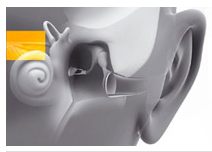
\includegraphics[width=45mm]{panp.png}
							\caption{Perda auditiva neurossensorial profunda unilateral. Fonte: Cochlear, 2012}
						\end{figure}
						
						É quando a perda auditiva é de grau profundo, ou seja, a audição é mínima ou nula, em \textbf{um dos ouvidos}, no outro a audição é normal. Possíveis causas: doenças, surdez súbita, congênita, tumor no nervo e lesão na cabeça.
						Essa perda auditiva é profunda e unilateral, faz com que o indivíduo seja incapaz de localizar de onde o som está vindo, há dificuldade de compreensão das conversas vindas do lado surdo. Em alguns casos, pode ser
						tratada com aparelhos auditivos ou sistema Baha.
						
					\item [-] \textbf{Central} 
											
						\begin{figure}[h]
							\center
							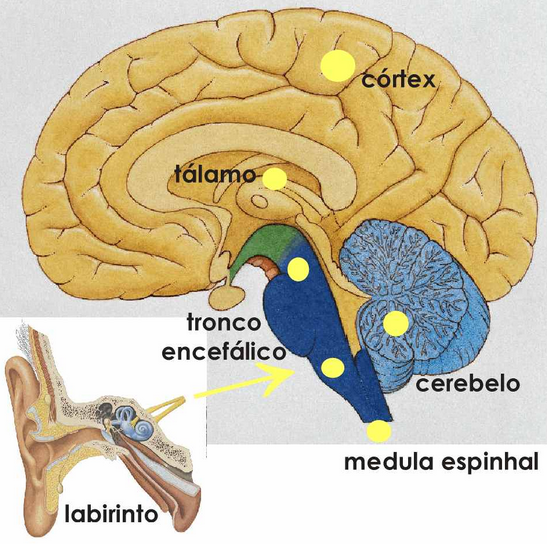
\includegraphics[width=5cm]{pace.png}
							\caption{Vertigem e tontura. Fonte: Pereira, 2012}
						\end{figure}
						
						É quando a alteração está localizada a partir do \textbf{tronco cerebral indo até as regiões subcorticais e córtex cerebral}, sendo que, não é, necessariamente, uma diminuição da sensibilidade auditiva. Entretanto, apresenta
						diferentes graus de dificuldade na percepção e compreensão dos sons. As perdas centrais são mais raras em crianças.
					
				\end{itemize}
					
									
			\subsection{Grau}
				O \textbf{grau} ou o nível de intensidade da perda auditiva pode ser classificado como:
							
				\begin{itemize}		
					\item [-] \textbf{Audição normal}
					
					Sem perda auditiva. Sem dificuldade aparente. Quanto a via aérea e a via óssea estão abaixo dos \textbf{20 decibéis}. 
					
					\item [-] \textbf{Deficiência auditiva leve} 
					
					Quem apresenta este grau de deficiência auditiva têm dificuldade para escutar à distância ou em ambientes ruidosos, 
					não provoca atraso na aquisição da linguagem e tem plenas condições de frequentar a escola comum. Porém, podem dificuldades 
					em ouvir a voz do professor. Na escola, essas crianças, são ditas como distraídas.
					Devem ter uma colocação adequada dentro da sala de aula, e um necessitam de um ensino de leitura de palavras e de estímulo 
					da linguagem. Quanto a via aérea e a via óssea possuem frequências entre \textbf{20 e 40 decibéis}.
										
					\item [-] \textbf{Moderada} 
					
					Quem apresenta este grau de deficiência não consegue acompanhar uma conversa normal se há ruído de fundo, pode apresentar 
					distúrbio articulatório (ausência ou produção inadequada dos sons orais), apresenta um aprendizado lento, pode ter algum grau de 
					isolamento e faz-se aqui o uso de leitura labial. Quanto a via aérea e a via óssea possuem frequências entre \textbf{40 e 70 decibéis}.
					
					\item [-] \textbf{Severa}
					
					Quem apresenta este grau de deficiência tem dificuldade em ouvir o que está sendo dito em quase todas as situações, necessitam 
					de uma prótese auditiva potente ou implante. Mesmo usando próteses tem dificuldade em distinguir vogais e consoantes. Na escola, apresentam
					algumas dificuldades psicológicas e na aquisição da linguagem. Precisam de cuidados especiais no treino da audição, na leitura de palavras e 
					estumulação da linguagem. Neste caso, muitos utilizam a linguagem gestual tanto para se expressar como para compreender. Quanto a via aérea 
					e a via óssea possuem frequências entre \textbf{70 e 90 decibéis}.
					
					\item [-] \textbf{Profunda}
					
					Neste, o indivíduo não possue nehuma sensação auditiva. Quem apresenta este grau de surdez, utiliza leitura labial e/ou linguagem gestual.
					Aqui, faz-se necessário métodos diferenciados para o estímulo e a aquisição da linguagem. Um dos possíveis tratamentos é o implante coclear.
					Quanto a via aérea e a via óssea possuem frequências superiores a \textbf{90 decibéis}.
					
				\end{itemize}
	

\chapter{O som e a estrutura do ouvido humano}
			O som pode ser descrito através de uma sequência de ondas sonoras, que são ondas de deslocamento, densidade e pressão que se propagam pelos meios compressíveis, ou seja,o som é um fenômeno resultante 
			da movimentação das partículas do ar. Sendo que, qualquer fato possível de causar ondas de pressão no ar é considerado um princípio sonoro.	Por exemplo a fala, é o resultado do movimento dos órgãos 
			fono-articulatórios, que provoca a movimentação das partículas de ar, produzindo então o som.
			
			Para melhor compreender a surdez devemos de início conhecer a anatomia da orelha humana.
				\begin{figure}[h]
					\center
					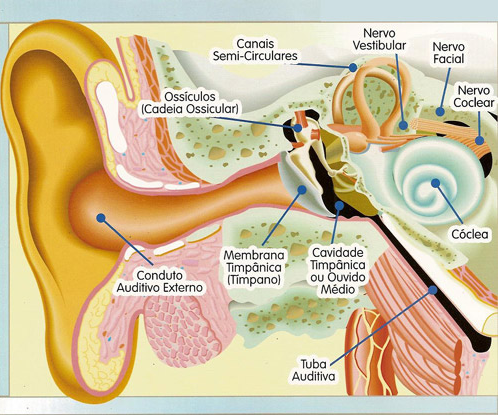
\includegraphics[width=58mm]{aa.png}
					\caption{Anatomia da orelha humana. Fonte: Audiológica, 2011}
				\end{figure}
			
			Identificar, captar, interpretar e absorver os diferentes sons em nossa volta só é possível devido à existência das três estruturas que funcionam em harmonia, o sistema auditivo humano.
			A anatomia do nosso ouvido é composta por três partes, uma externa e outras duas internas (localizadas dentro da caixa craniana), de acordo com a Audiológica e o documento escrito pelo MEC, 
			Saberes e práticas da inclusão: Desenvolvendo competências para o atemdimento às necessidades educacionais especiais de alunos surdos:
			
				\begin{figure}[!htb]
					\center
					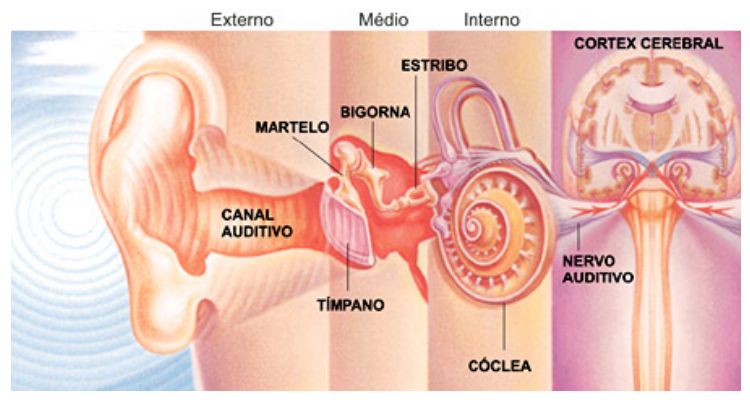
\includegraphics[width=95mm]{aa2.png}
					\caption{Anatomia da orelha humana. Fonte: Audição em mamíferos, 2011}
				\end{figure}
				
				\begin{itemize}		
					\item [-]\textbf{Ouvido externo:}
					
					{ No ouvido externo, na parte externa, se encontram o pavilhão auricular (orelha), o meato acústico externo e a menbrana timpânica. Por sua vez, a função da parte externa é localizar e 
					juntar as ondas sonoras, captadas pela orelha e levar para o meato acústico que os encaminha até a membrana timpânica. A menbrana timpânica separa o ouvido externo e o ouvido médio.
					É também no canal auditivo que se dá a produção de cera, que é uma forma de manter húmido e limpo o ouvido. Pois, a cera ajuda a reter partículas de pó, sujidade e microorganismos.} 
			
					\item[-]\textbf{Ouvido médio:}
					
					{ No ouvido médio, ou cavidade timpânica, encontra-se a cadeia ossicular, determinada pelo martelo, a bigorna e o estribo. Esses ossículos são presos por músculos, que tem a função de 
					transmitir e limitar a energia sonora para a orelha interna, algo fundamental para evitar danos no ouvido interno quando estamos expostos a sons de intensidade elevada. Neste, se 
					encontra também a tuba auditiva, que tem como finalidade o equilíbrio da pressão entre os ouvidos médios e externos, e que faz a ligação do ouvido à garganta.}
					
					\item[-]\textbf{Ouvido interno:}
					
					{ No ouvido interno, está localizada a cóclea (que tem formato de caracol) e o labirinto (ou canais semicirculares, responsáveis pelo equilíbrio). É nessa etapa que ocorre a percepção dos som.
					Este trajeto é preenchido por líquidos que ao se deslocarem, movem as células responsáveis pela geração dos impulsos nervosos transmitidos ao cérebro pelo nervo auditivo. No cérebro, os impulsos 
					nervosos são assimilados, compreendidos e distinguidos pelos córtex auditivo.}				
				\end{itemize}
				
			Entendido o sistema auditivo humano, qualquer que seja a alteração ou distúrbio no processamento da audição é considerada uma alteração auditiva, fazendo com que o indivíduo tenha um decréscimo da 
			sua capacidade de ouvir e compreender o som.

\chapter{Audiometria}
	Quanto ao grau ou ao nível de surdez, os testes auditivos podem medir a quantidade de som que você pode ou não pode ouvir. 
	Os resultados dos testes de audição podem ser exibidos em um gráfico chamado de \textbf{audiograma}.

	O teste de audição serve para detectar se há algum problema auditivo, qual a possível causa da perda auditiva e também para auxiliar o médico numa melhor opção de tratamento.
	Sendo este medido em decibéis (dB). Este número indica o quão forte deve ser o som que você pode ouvir em comparação com pessoas com audição normal. A \textbf{audiometria} serve para avaliar 
	a condução por via aérea e via óssea do som.
				
		\begin{itemize}
		
			\item [-] \textbf{Via aérea}
				\begin{figure}[!htb]
					\center
					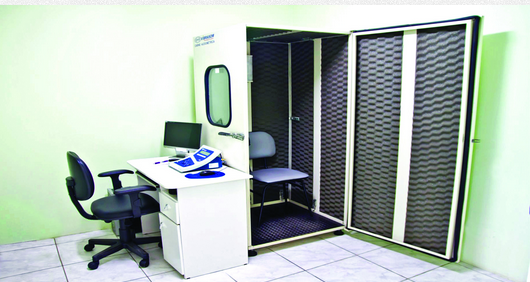
\includegraphics[width=65mm]{ava.png}
					\caption{Audiometria. Fonte: Vetro Serra}
				\end{figure}
					
			Esta pesquisa é ralizada nas frequências de 0,25 Hz a 8 kHz. Os estímulos auditivos podem ser feitos por meio de fones de ouvido ou caixa de som. 

			\item [-] \textbf{Via óssea}
				\begin{figure}[!htb]
					\center
					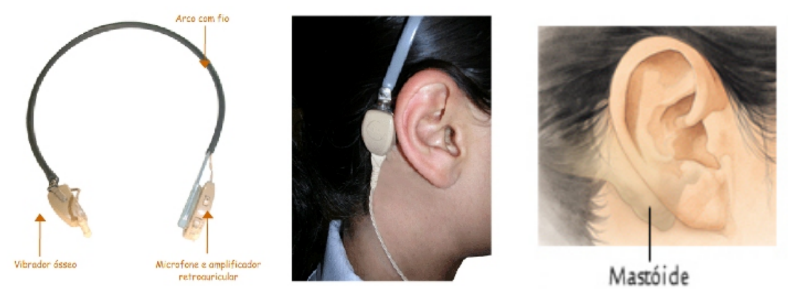
\includegraphics[width=95mm]{mvo.png}
					\caption{Condução óssea. Fonte: Portal dos bebês}
				\end{figure}
											
			Para este tipo de avaliação é utilizado um vibrador ósseo posicionado na mastóide, que não deverá encostar no pavilhão auricular (orelha). Esta pesquisa é feita nas frequências de 0,5 Hz a 4 kHz. Esta serve para avaliar a capacidade de detectar 
			sons transmitidos através dos ossos da cabeça. 
					
		\end{itemize}			
    
\end{document}
    
\bibliographystyle{abnt-num}
